\section{Introduction}\label{s:intro}

Most supervised deep learning methods require large quantities of manually labelled data, limiting their applicability in many scenarios.
This is true for large-scale image classification and even more for segmentation (pixel-wise classification) where the annotation cost per image is very high~\cite{lin2014microsoft,girshick2014rich}.
Unsupervised clustering, on the other hand, aims to group data points into classes entirely without labels~\cite{hartigan1972direct}.
Many authors have sought to combine mature clustering algorithms with deep learning, for example by bootstrapping network training with k-means style objectives~\cite{xie2016unsupervised, haeusser2018associative, caron2018deep}.
%by learning deep feature representations in an unsupervised fashion (context prediction~\cite{doersch2015unsupervised}, exemplars~\cite{dosovitskiy2014discriminative}) followed by k-means in post-processing, or by bootstrapping network training using k-means itself~\cite{caron2018deep, xie2016unsupervised}.
However, trivially combining clustering and representation learning methods often leads to degenerate solutions~\cite{caron2018deep, xie2016unsupervised}.
It is precisely to prevent such degeneracy that cumbersome pipelines --- involving pre-training, feature post-processing (whitening or PCA), clustering mechanisms external to the network --- have evolved~\cite{caron2018deep,doersch2015unsupervised,dosovitskiy2015discriminative,xie2016unsupervised}.

%\begin{figure}[t]
\centering
\bgroup
\def\arraystretch{1.8}
\begin{tabular}{c c c c c c c c c c c c}

\multicolumn{4}{c}{
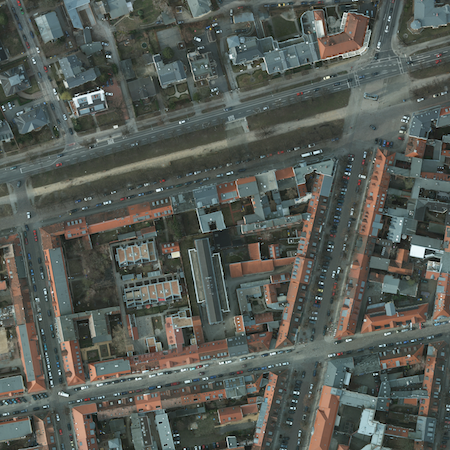
\includegraphics[height=0.277\textwidth]{experiments2_files/545_17_img.png}} & 
\multicolumn{4}{c}{
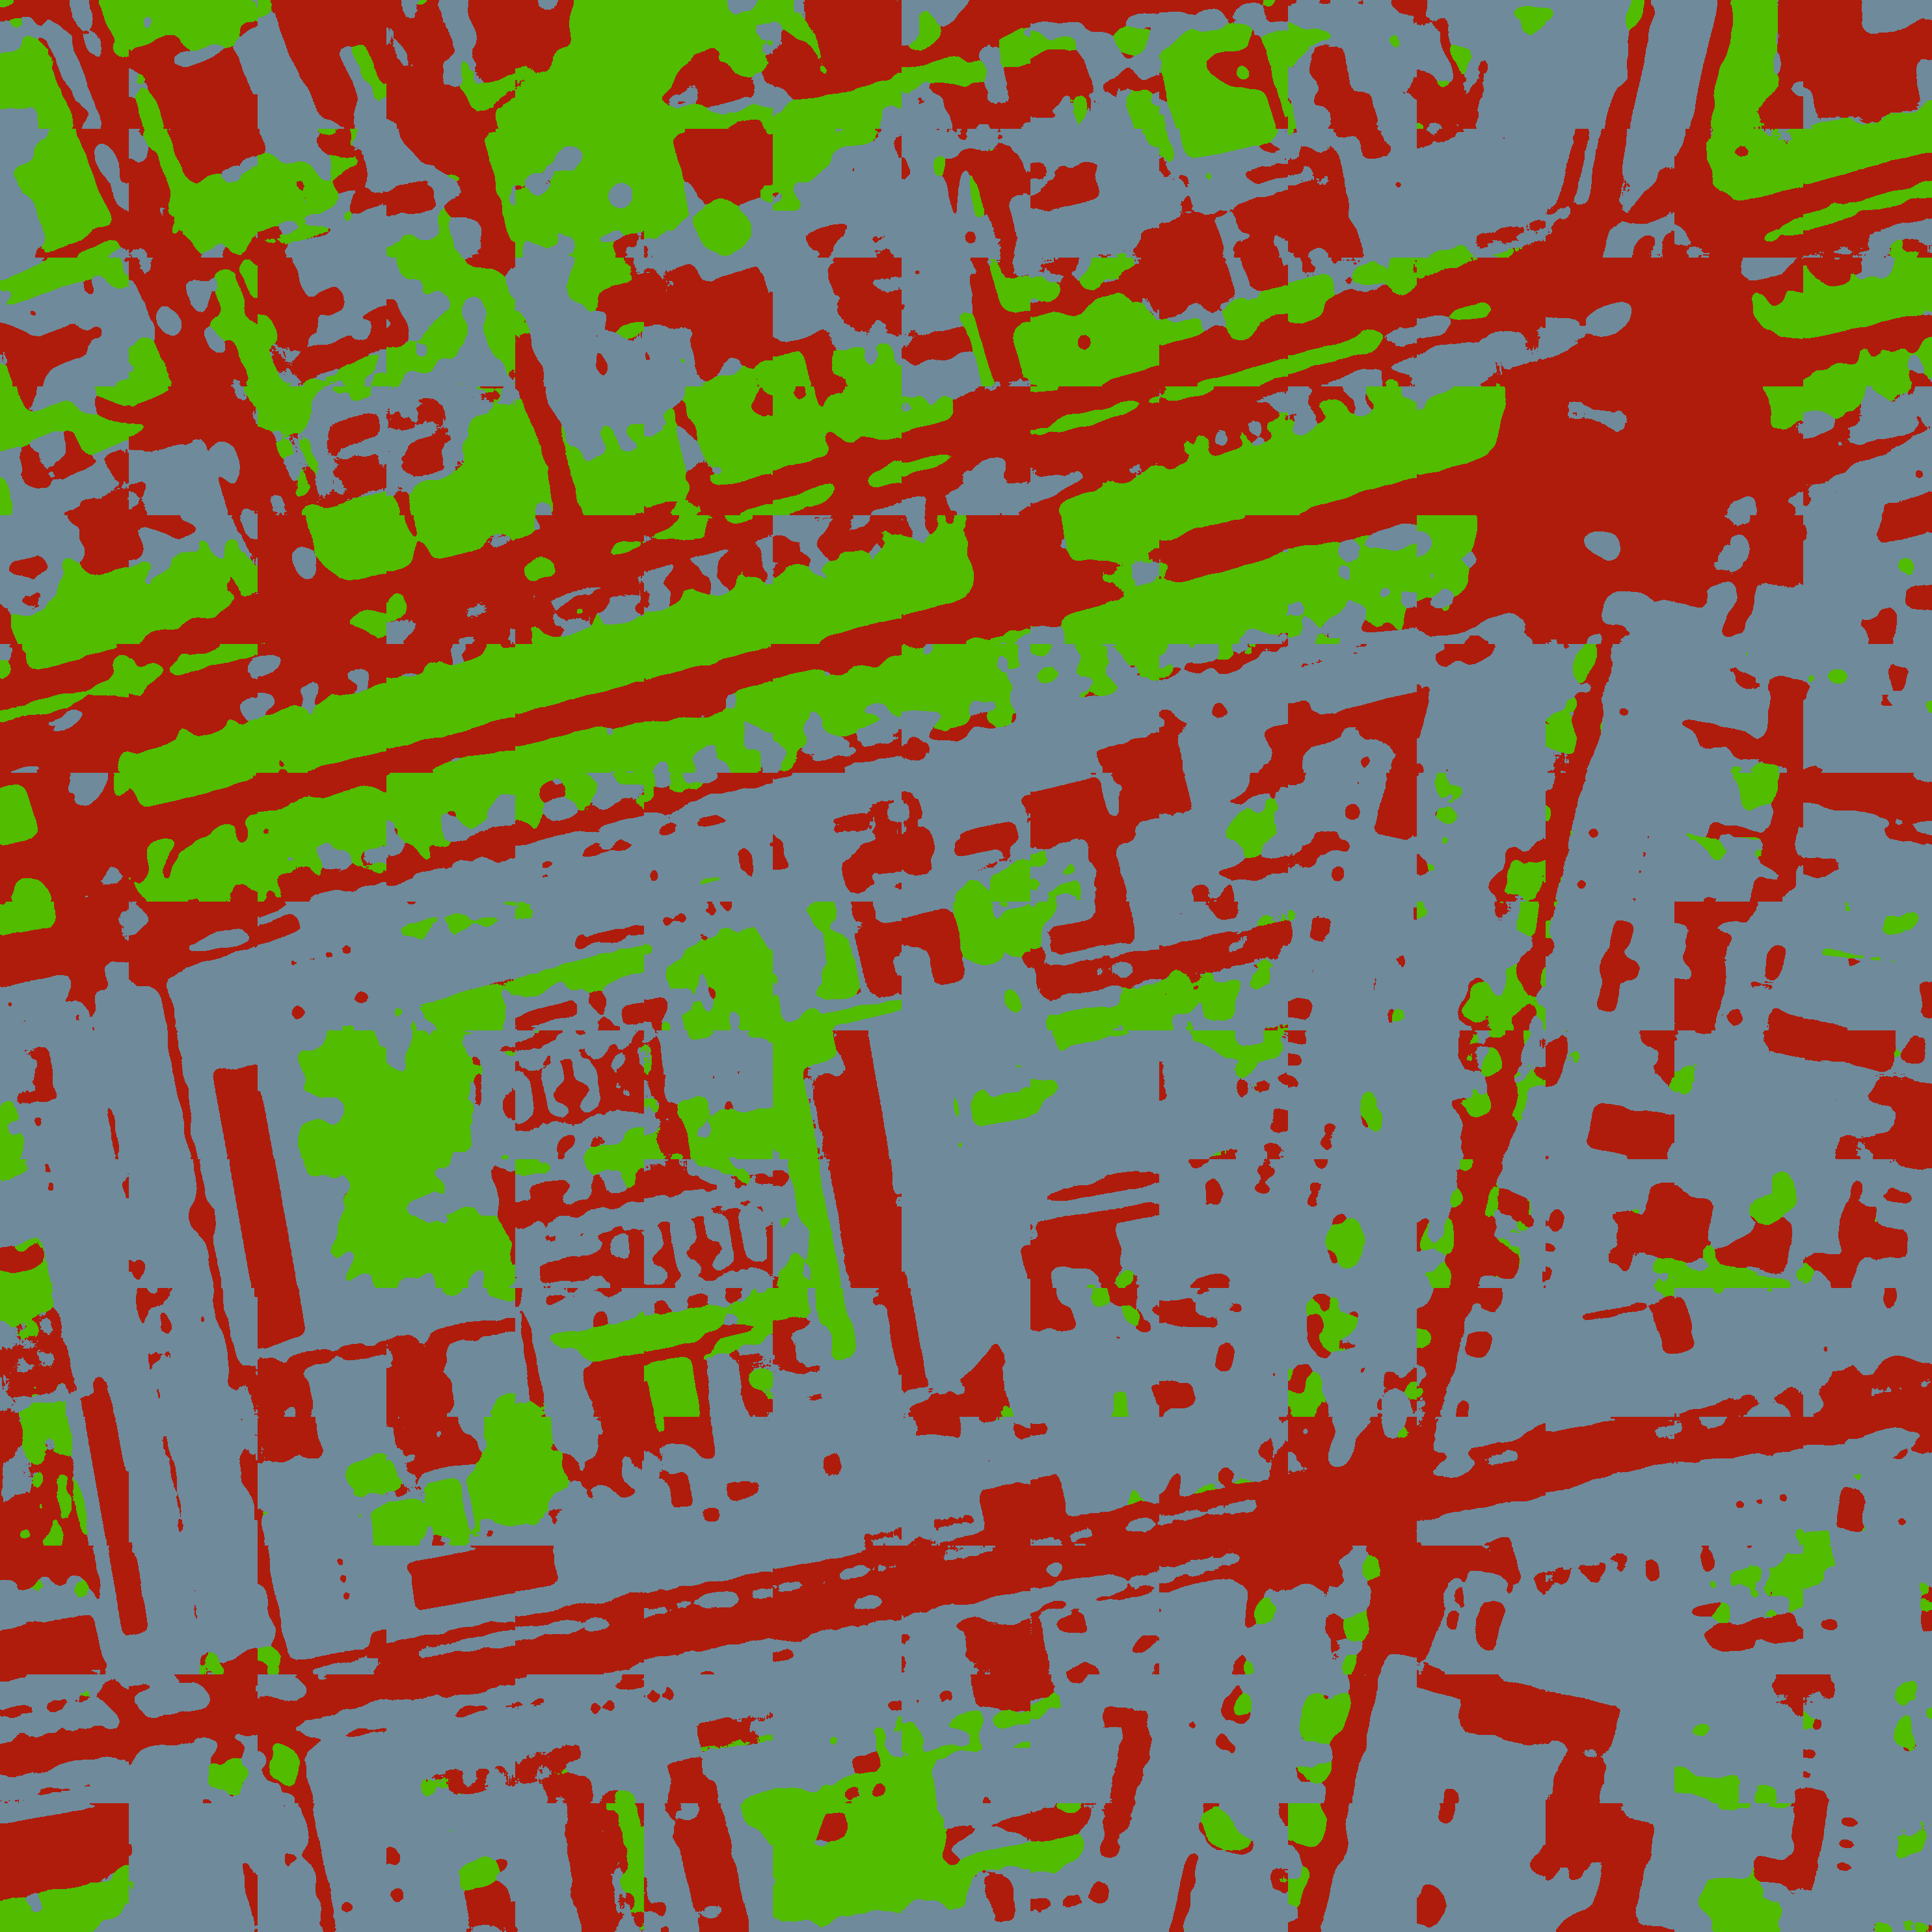
\includegraphics[height=0.277\textwidth]{experiments2_files/545_17_preds.png}} & 
\multicolumn{4}{c}{
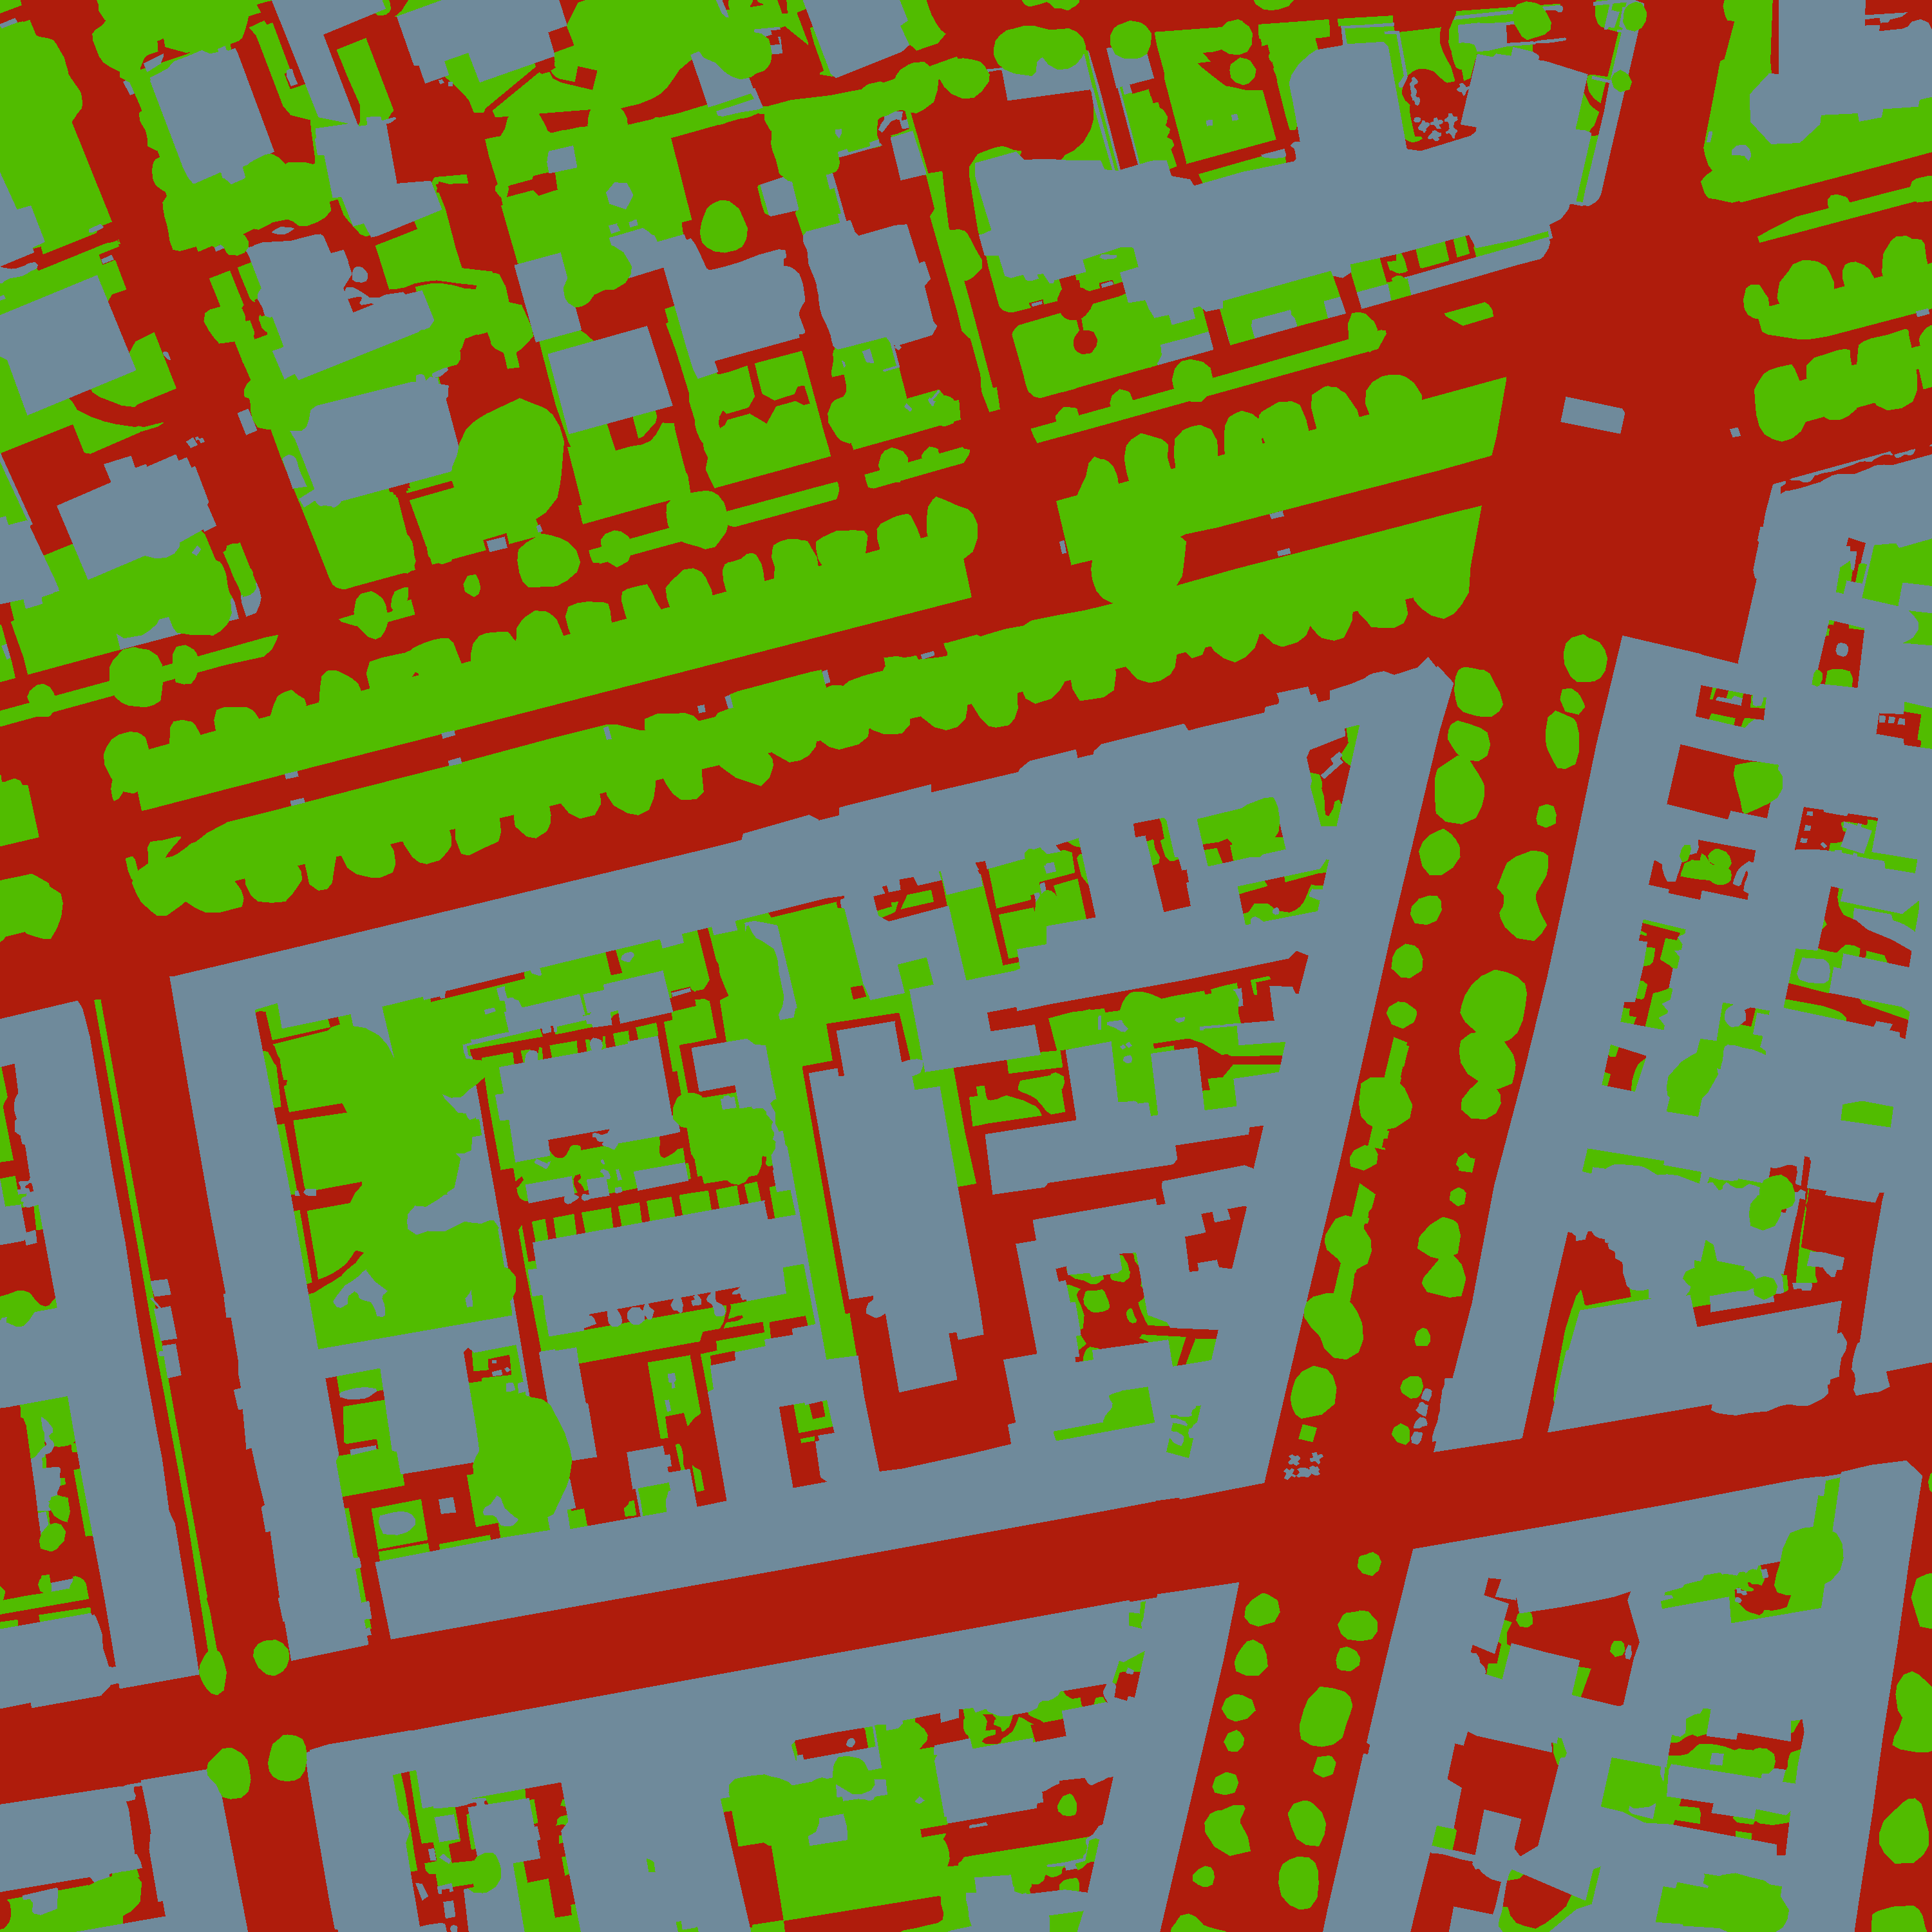
\includegraphics[height=0.277\textwidth]{experiments2_files/545_17_gt.png}} \\

\multicolumn{4}{c}{
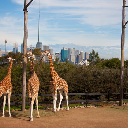
\includegraphics[height=0.277\textwidth]{experiments2_files/509_img_254.png}} & 
\multicolumn{4}{c}{

\includegraphics[height=0.277\textwidth]{experiments2_files/509_reordered_preds_254.png}} & 
\multicolumn{4}{c}{

\includegraphics[height=0.277\textwidth]{experiments2_files/509_targets_254.png}} \\

\multicolumn{3}{c}{
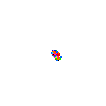
\includegraphics[height=0.20\textwidth]{experiments2_files/556_pointcloud_random.png}} & 
\multicolumn{3}{c}{
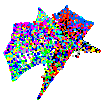
\includegraphics[height=0.20\textwidth]{experiments2_files/556_pointcloud_e_3.png}} & 
\multicolumn{3}{c}{
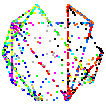
\includegraphics[height=0.20\textwidth]{experiments2_files/556_pointcloud_e_24.png}} &
\multicolumn{3}{c}{
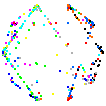
\includegraphics[height=0.20\textwidth]{experiments2_files/247_pointcloud_best.png}}\\

\end{tabular}
\egroup
\caption{\label{f:splash} Fully unsupervised image clustering and segmentation (IID). Top: input, prediction and ground truth for Potsdam-3 and COCO-Stuff-3. Bottom: raw STL10 predictions before, during and after training.}
\end{figure}

\begin{figure}[t]

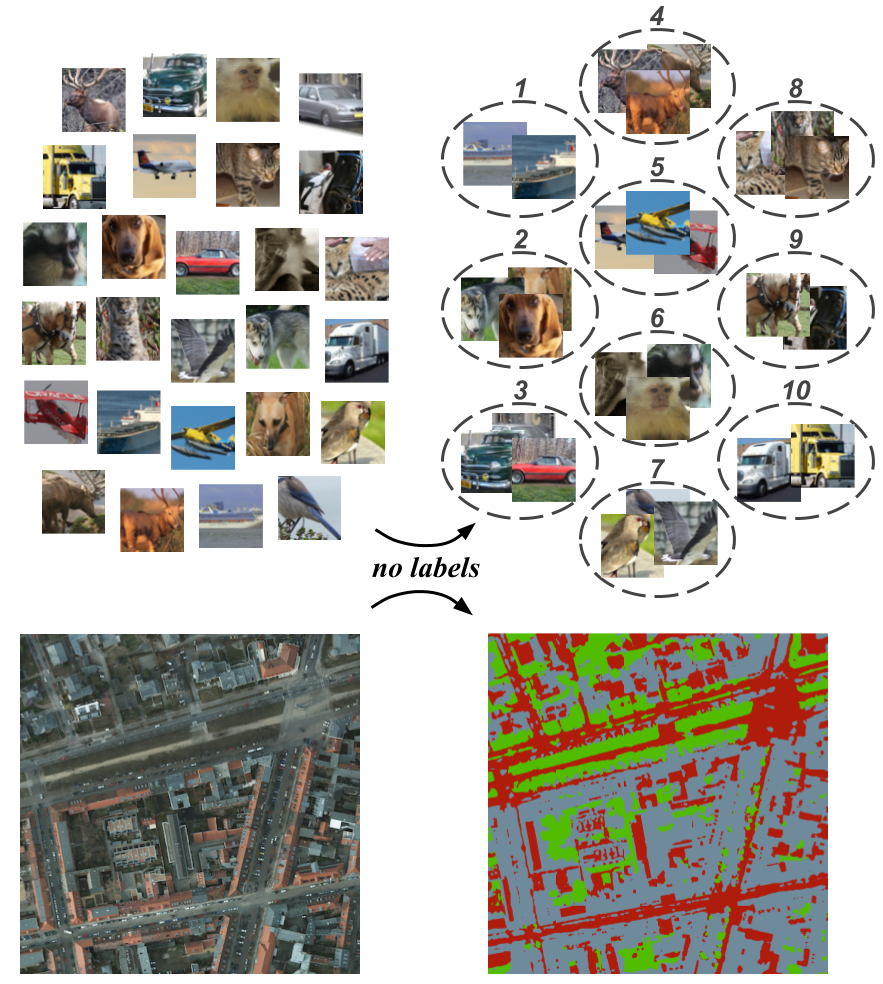
\includegraphics[height=1.1\textwidth]{experiments2_files/splash2.png}

\caption{\label{f:splash} Models trained with \methodnameshort on entirely unlabelled data learn to cluster images (top, STL10) and patches (bottom, Potsdam-3). The raw clusters found directly correspond to semantic classes (dogs, cats, trucks, roads, vegetation etc.) with state-of-the-art accuracy.  Training is end-to-end and randomly initialised, with no heuristics used at any stage.}
\end{figure}


In this paper, we introduce \methodname (\methodnameshort), a method that addresses this issue in a more principled manner.
\methodnameshort is a generic clustering algorithm that directly trains a randomly initialised neural network into a classification function, end-to-end and without any labels.
It involves a simple objective function, which is the mutual information between the function's classifications for paired data samples. The input data can be of any modality and, since the clustering space is discrete, mutual information can be computed exactly.

Despite its simplicity, \methodnameshort is intrinsically robust to two issues that affect other methods.
The first is clustering degeneracy, which is the tendency for a single cluster to dominate the predictions or for clusters to disappear (which can be observed with k-means, especially when combined with representation learning~\cite{caron2018deep}).
Due to the entropy maximisation component within mutual information, the loss is not minimised if all images are assigned to the same class. At the same time, it is optimal for the model to predict for each image a single class with certainty (i.e. one-hot) due to the conditional entropy minimisation~(\cref{f:mnist_dots}). The second issue is noisy data with unknown or distractor classes (present in STL10~\cite{coates2011analysis} for example).
\methodnameshort addresses this issue by employing an auxiliary output layer that is parallel to the main output layer, trained to produce an overclustering (i.e.\ same loss function but greater number of clusters than the ground truth) that is ignored at test time.
Auxiliary overclustering is a general technique that could be useful for other algorithms.
These two features of \methodnameshort contribute to making it the only method amongst our unsupervised baselines that is robust enough to make use of the noisy unlabelled subset of STL10, a version of ImageNet~\cite{deng2009imagenet} specifically designed as a benchmark for unsupervised clustering.

In the rest of the paper, we begin by explaining the difference between semantic clustering and intermediate representation learning~(\cref{s:related}), which separates our method from the majority of work in unsupervised deep learning. 
We then describe the theoretical foundations of \methodnameshort in statistical learning~(\cref{s:method}), demonstrating that maximising mutual information between pairs of samples under a bottleneck is a principled clustering objective which is equivalent to distilling their shared abstract content (co-clustering).
We propose that for static images, an easy way to generate pairs with shared abstract content from unlabelled data is to take each image and its random transformation, or each patch and a neighbour.
We show that maximising MI automatically avoids degenerate solutions and can be written as a convolution in the case of segmentation, allowing for efficient implementation with any deep learning library.

We perform experiments on a large number of datasets~(\cref{s:experiments}) including STL, CIFAR, MNIST, COCO-Stuff and Potsdam, setting a new state-of-the-art on unsupervised clustering and segmentation in all cases, with results of 59.6\%, 61.7\% and 72.3\% on STL10, CIFAR10 and COCO-Stuff-3 beating the closest competitors (53.0\%, 52.2\%, 54.0\%) with significant margins.
Note that training deep neural networks to perform large scale, real-world segmentations from scratch, without labels or heuristics, is a highly challenging task with negligible precedent.
%Note that training deep neural networks to cluster large scale, real-world datasets from scratch and without labels is extremely challenging and is still the subject of very active research.
%has been addressed comparatively rarely in the literature.
%real-world datasets with neither labels nor heuristics is extremely challenging and has been addresses comparatively rarely in the literature.
%negligible precedent.
We also perform an ablation study and additionally test two semi-supervised modes, setting a new global state-of-the-art of 88.8\% on STL10 over all supervised, semi-supervised and unsupervised methods, and demonstrating the robustness in semi-supervised accuracy when 90\% of labels are removed.


